\documentclass[conference]{IEEEtran}
\IEEEoverridecommandlockouts
\usepackage[brazilian]{babel}
\usepackage[utf8]{inputenc}
\usepackage[T1]{fontenc}
\usepackage{cite}
\usepackage{amsmath,amssymb}
\usepackage{graphicx}
\usepackage{booktabs}
\usepackage{xcolor}
\usepackage{url}
\usepackage[hidelinks]{hyperref}

% Números gerados automaticamente por main.py (paper/generated/macros.tex)
% Gerado automaticamente por main.py -- não editar à mão
\newcommand{\NTotalFiles}{3829}
\newcommand{\NAugExcluded}{2931}
\newcommand{\NGroups}{781}
\newcommand{\NNearDup}{144}
\newcommand{\NDuplicates}{31}
\newcommand{\NConflicting}{0}
\newcommand{\NCorrupt}{0}
\newcommand{\NClean}{867}
\newcommand{\NClasses}{6}
\newcommand{\NTrain}{607}
\newcommand{\NVal}{124}
\newcommand{\NTest}{136}
\newcommand{\BestLabel}{ViT-B/16 com DA}
\newcommand{\AccResNetAug}{91.91}
\newcommand{\FOneResNetAug}{89.49}
\newcommand{\ErrorsResNetAug}{11}
\newcommand{\BestEpochResNetAug}{13}
\newcommand{\AccResNetNoAug}{88.97}
\newcommand{\FOneResNetNoAug}{84.48}
\newcommand{\ErrorsResNetNoAug}{15}
\newcommand{\BestEpochResNetNoAug}{12}
\newcommand{\AccViTAug}{94.85}
\newcommand{\FOneViTAug}{91.46}
\newcommand{\ErrorsViTAug}{7}
\newcommand{\BestEpochViTAug}{14}
\newcommand{\AccViTNoAug}{91.91}
\newcommand{\FOneViTNoAug}{87.45}
\newcommand{\ErrorsViTNoAug}{11}
\newcommand{\BestEpochViTNoAug}{8}
\newcommand{\DeltaAugResNet}{+5.01}
\newcommand{\DeltaAugViT}{+4.01}
\newcommand{\BestAcc}{94.85}
\newcommand{\BestFOne}{91.46}
\newcommand{\NCommonErrors}{5}
\newcommand{\TopConfTrue}{Leaf scald}
\newcommand{\TopConfPred}{Brown Spot}
\newcommand{\TopConfN}{3}


% Trechos em vermelho = interpretação que depende do resultado real.
% Leia depois de rodar os experimentos, ajuste se preciso e troque
% \revisar{...} por texto normal (ou redefina abaixo como #1).
\newcommand{\revisar}[1]{\textcolor{red}{#1}}

\begin{document}

\title{Classificação de Doenças em Folhas de Arroz com CNN e \textit{Vision Transformer}:
uma Análise do Impacto do \textit{Data Augmentation}}

\author{\IEEEauthorblockN{Vinícius Matoso Dias\\
Paulo Roberto\\
Gabriel Rodrigues}
\IEEEauthorblockA{Sistemas de Informação\\
Universidade Federal de Viçosa -- Campus Rio Paranaíba\\
Rio Paranaíba, MG, Brasil\\
vinicius.matoso@ufv.br}
}

\maketitle

\begin{abstract}
Doenças foliares estão entre as principais causas de perda de produtividade na cultura do arroz, e o diagnóstico visual depende de especialistas nem sempre disponíveis no campo. Este trabalho avalia a classificação automática de \NClasses{} condições de folhas de arroz (cinco doenças e folha saudável) a partir de imagens RGB do \textit{Rice Disease Dataset}, disponível no Kaggle. Foram comparadas uma rede convolucional (ResNet-50) e um \textit{Vision Transformer} (ViT-B/16), ambos inicializados com pesos do ImageNet e ajustados por completo, cada um treinado com e sem \textit{data augmentation}, totalizando quatro experimentos sob a mesma divisão estratificada treino/validação/teste. Uma inspeção do conjunto revelou que a maior parte dos arquivos são cópias geradas por \textit{data augmentation} offline das fotos originais; elas foram descartadas e as quase-duplicatas restantes foram agrupadas antes da divisão, para evitar vazamento de dados entre treino e teste. O melhor resultado no conjunto de teste foi obtido pelo modelo \BestLabel{}, com acurácia de \BestAcc\% e F1-macro de \BestFOne\%. São discutidos o efeito do \textit{data augmentation} em cada arquitetura, as classes mais confundidas e as possíveis causas dos erros.
\end{abstract}

\begin{IEEEkeywords}
visão computacional, aprendizado profundo, doenças do arroz, ResNet, \textit{Vision Transformer}, \textit{data augmentation}
\end{IEEEkeywords}

% =====================================================================
\section{Introdução}
O arroz (\textit{Oryza sativa}) é alimento básico para grande parte da população mundial, e doenças como a brusone (\textit{leaf blast}), a mancha-parda (\textit{brown spot}), a queima-das-bainhas (\textit{sheath blight}), a escaldadura (\textit{leaf scald}) e a queima bacteriana (\textit{bacterial leaf blight}) reduzem a produtividade e a qualidade dos grãos. O diagnóstico costuma ser feito por inspeção visual, um processo lento, subjetivo e dependente de especialistas. A classificação automática de imagens de folhas é, por isso, uma aplicação natural de visão computacional na agricultura de precisão.

Redes neurais convolucionais (CNNs) dominam essa tarefa há quase uma década, mas arquiteturas baseadas em atenção, como o \textit{Vision Transformer} (ViT)~\cite{dosovitskiy2021vit}, passaram a disputar o estado da arte em classificação de imagens. Como os ViTs possuem menos vieses indutivos que as CNNs (localidade e invariância à translação), eles tendem a depender mais de dados e de regularização, o que torna relevante investigar como cada família se comporta em um conjunto de dados agrícola de tamanho moderado e qual o papel do \textit{data augmentation} nesse cenário.

Este trabalho investiga duas questões experimentais: (Q1)~qual arquitetura, ResNet-50~\cite{he2016resnet} ou ViT-B/16~\cite{dosovitskiy2021vit}, ambas com \textit{transfer learning} do ImageNet~\cite{deng2009imagenet}, apresenta melhor desempenho na classificação de doenças em folhas de arroz; e (Q2)~qual o impacto do \textit{data augmentation} em cada uma delas. O restante do artigo está organizado da seguinte forma: a Seção~\ref{sec:revisao} revisa trabalhos relacionados; a Seção~\ref{sec:metodos} descreve o conjunto de dados e o protocolo experimental; a Seção~\ref{sec:resultados} apresenta e discute os resultados; e a Seção~\ref{sec:conclusao} conclui o trabalho.

% =====================================================================
\section{Revisão Bibliográfica}\label{sec:revisao}
Ahad et al.~\cite{ahad2023comparison} compararam seis arquiteturas CNN (DenseNet121, InceptionV3, MobileNetV2, ResNeXt101, ResNet152V2 e SEResNeXt101) na classificação de nove doenças do arroz. Os autores relatam acurácia de até 98\% e mostram que o \textit{transfer learning} elevou em cerca de 17 pontos percentuais a acurácia do SEResNeXt101 em relação ao treinamento a partir do zero, evidenciando o valor de pesos pré-treinados quando há poucos dados.

Simhadri e Kondaveeti~\cite{simhadri2023automatic} avaliaram 15 CNNs pré-treinadas com \textit{transfer learning} para o reconhecimento de doenças foliares do arroz, obtendo os melhores resultados com a InceptionV3 (acurácia média de 99,64\%). O estudo reforça que arquiteturas convolucionais consolidadas, quando ajustadas ao problema, atingem desempenho elevado em conjuntos de dados controlados.

Entre os trabalhos com atenção, Pavithra e Baranidharan~\cite{pavithra2024hybrid} propuseram um modelo híbrido ViT-CNN que insere blocos convolucionais dentro das camadas do \textit{transformer} para identificar cinco doenças do arroz, reportando precisão de 93,84\% e desempenho superior a \textit{transformers} puros. Na mesma linha, Sennan et al.~\cite{sennan2025hybrid} combinaram as características extraídas por um ViT e por uma ResNet18 pré-treinada em uma camada totalmente conectada comum, explorando a complementaridade entre o contexto global da atenção e as características locais das convoluções.

Mehnaz e Islam~\cite{mehnaz2025comparative} compararam diretamente CNNs (ResNet50, ResNet152 e InceptionV3), um \textit{transformer} (MaxViT) e SVM no conjunto Dhan-Shomadhan. A ResNet50 obteve 91,5\% de acurácia contra 75,0\% do MaxViT, um resultado que sugere que, com poucos dados, CNNs pré-treinadas podem superar \textit{transformers}, o que motiva a questão Q1 deste trabalho. Rimi et al.~\cite{rimi2025riceleafbd} apresentaram o conjunto RiceLeafBD e compararam uma CNN leve com InceptionNet-V2, EfficientNet-V2 e MobileNet-V2, com melhor acurácia de 91,5\% para a EfficientNet-V2.

Por fim, Prity et al.~\cite{prity2025neural} utilizaram imagens das mesmas seis classes adotadas aqui (queima bacteriana, mancha-parda, brusone, escaldadura, queima-das-bainhas e folha saudável) e compararam um modelo baseado em extração e seleção de características com \textit{Extreme Learning Machine} a um modelo que recebe as imagens diretamente, com validação cruzada de 10 partições.

Diferentemente desses trabalhos, que em geral propõem uma arquitetura ou comparam várias CNNs, este estudo realiza uma comparação controlada entre uma CNN e um ViT puros, com os mesmos hiperparâmetros, e isola o efeito do \textit{data augmentation} em cada arquitetura, além de identificar e tratar a presença de imagens aumentadas e quase-duplicadas no conjunto público, que levaria a vazamento entre treino e teste.

% =====================================================================
\section{Material e Métodos}\label{sec:metodos}

\subsection{Conjunto de dados}
Foi utilizado o \textit{Rice Disease Dataset}~\cite{kaggle_rice}, disponível publicamente no Kaggle, composto por imagens RGB de folhas de arroz organizadas em \NClasses{} classes: \textit{Bacterial Leaf Blight}, \textit{Brown Spot}, \textit{Healthy Rice Leaf}, \textit{Leaf Blast}, \textit{Leaf Scald} e \textit{Sheath Blight}. Exemplos de cada classe são mostrados na Fig.~\ref{fig:amostras}.

O conjunto contém \NTotalFiles{} arquivos na pasta \texttt{Rice\_Leaf\_AUG}. Uma inspeção dos nomes e resoluções mostrou que \NAugExcluded{} deles (nomeados \texttt{aug\_0\_*.jpg}, todos com $224\times224$ pixels) são versões transformadas (rotações, espelhamentos, recortes) das fotos originais, geradas pelo autor do conjunto, enquanto as fotos originais têm resoluções de câmera (por exemplo, $1600\times1200$ ou $4000\times3000$). Essas cópias foram descartadas por dois motivos: (i)~com uma divisão aleatória, versões da mesma foto cairiam no treino e no teste, e o modelo seria avaliado em imagens praticamente já vistas, inflando as métricas (vazamento de dados); e (ii)~manter um conjunto já aumentado tornaria sem sentido a questão Q2, que mede justamente o efeito do \textit{data augmentation}.

Em seguida, as fotos restantes foram verificadas quanto à integridade (\NCorrupt{} corrompidas) e duplicatas exatas foram identificadas pelo \textit{hash} MD5: foram removidas \NDuplicates{} cópias redundantes (por exemplo, arquivos ``\texttt{- Copy}'') e \NConflicting{} imagens idênticas presentes em classes diferentes, restando \NClean{} imagens. Por fim, como o conjunto contém fotos tiradas em sequência da mesma folha, foi calculado um \textit{hash} perceptual (dHash) de cada imagem nas oito orientações obtidas por rotações de $90^\circ$ e espelhamento; imagens da mesma classe com distância de Hamming $\le 6$ (em 64 bits) foram agrupadas, resultando em \NGroups{} grupos (\NNearDup{} imagens pertencem a grupos com mais de uma foto). A Tabela~\ref{tab:dataset} mostra que as classes são desbalanceadas, o que motiva a escolha do F1-macro como métrica principal.

\begin{figure}[t]
\centering
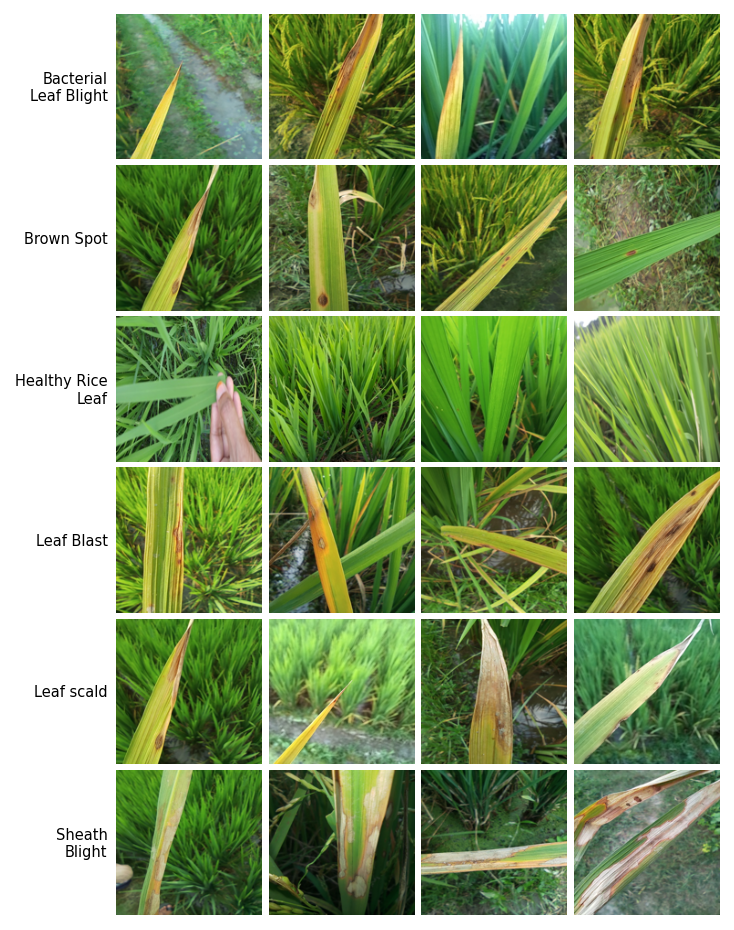
\includegraphics[width=0.85\columnwidth]{figures/dataset_samples.png}
\caption{Exemplos de imagens de cada classe do conjunto de treino.}
\label{fig:amostras}
\end{figure}

\subsection{Divisão dos dados}
Como o conjunto não é previamente dividido, aplicou-se a divisão \textit{hold-out} estratificada por classe com a função \texttt{train\_test\_split} do scikit-learn~\cite{pedregosa2011sklearn} e semente fixa (42), em duas etapas: primeiro foram separados 15\% para teste e, do restante, 15\% do total para validação, resultando em aproximadamente 70\%/15\%/15\% (\NTrain{}/\NVal{}/\NTest{} imagens). A divisão foi feita sobre os grupos de quase-duplicatas, e não sobre imagens individuais, de modo que fotos quase idênticas sempre ficam no mesmo conjunto. A Tabela~\ref{tab:dataset} mostra a distribuição por classe. O conjunto de validação foi usado para seleção do modelo e \textit{early stopping}; o conjunto de teste foi usado uma única vez, na avaliação final.

\begin{table}[t]
\centering
\caption{Distribuição das imagens por classe e conjunto após a limpeza.}
\label{tab:dataset}
\begin{tabular}{lcccc}
\toprule
Classe & Treino & Validação & Teste & Total \\
\midrule
Bacterial Leaf Blight & 62 & 13 & 14 & 89 \\
Brown Spot & 98 & 20 & 23 & 141 \\
Healthy Rice Leaf & 126 & 27 & 31 & 184 \\
Leaf Blast & 68 & 13 & 12 & 93 \\
Leaf scald & 56 & 10 & 10 & 76 \\
Sheath Blight & 197 & 41 & 46 & 284 \\
\midrule
Total & 607 & 124 & 136 & 867 \\
\bottomrule
\end{tabular}
\end{table}


\subsection{Pré-processamento e \textit{data augmentation}}
Todas as imagens foram redimensionadas para $224\times224$ pixels, resolução nativa dos pesos pré-treinados de ambos os modelos, e normalizadas com a média e o desvio padrão do ImageNet. Optou-se por redimensionar a imagem inteira em vez de aplicar recorte central, para não descartar lesões próximas às bordas da folha.

As transformações de \textit{data augmentation}~\cite{shorten2019survey}, aplicadas apenas ao treino e sorteadas a cada época, foram escolhidas para simular variações plausíveis de captura em campo sem alterar o rótulo:
\begin{itemize}
\item \textbf{Recorte e redimensionamento aleatórios} (escala de 70\% a 100\% da área): simulam distâncias e enquadramentos diferentes da câmera; o limite inferior evita cortar a região da lesão.
\item \textbf{Espelhamentos horizontal e vertical e rotação de até $\pm20^\circ$}: a orientação da folha na foto é arbitrária e não tem relação com a doença.
\item \textbf{Variação de cor leve} (brilho, contraste e saturação de $\pm20\%$; matiz de $\pm0{,}02$): simula iluminação natural (sol, sombra, céu nublado). A matiz varia muito pouco porque a cor é um sintoma diagnóstico, por exemplo as manchas marrons da \textit{Brown Spot} contra o verde da folha saudável, e alterá-la muito poderia gerar exemplos com rótulo incorreto.
\end{itemize}
Nos experimentos sem \textit{data augmentation}, o treino recebeu apenas o redimensionamento e a normalização.

\subsection{Modelos}
Foram utilizados dois modelos do \texttt{torchvision}, ambos com pesos pré-treinados no ImageNet-1k:
\begin{itemize}
\item \textbf{ResNet-50}~\cite{he2016resnet}: CNN de 50 camadas com conexões residuais, representante da família convolucional. A camada totalmente conectada final foi substituída por uma com \NClasses{} saídas.
\item \textbf{ViT-B/16}~\cite{dosovitskiy2021vit}: divide a imagem em \textit{patches} de $16\times16$ pixels, projetados como \textit{tokens} e processados por 12 blocos de autoatenção multi-cabeça. A cabeça de classificação foi substituída por uma camada linear com \NClasses{} saídas.
\end{itemize}
Em ambos os casos foi realizado ajuste fino (\textit{fine-tuning}) de todos os parâmetros.

\subsection{Treinamento}
Os quatro experimentos usaram exatamente os mesmos hiperparâmetros: perda de entropia cruzada, otimizador AdamW~\cite{loshchilov2019adamw} com taxa de aprendizado inicial de $10^{-4}$ e \textit{weight decay} de $10^{-4}$, decaimento cossenoidal da taxa de aprendizado, lotes de 32 imagens, no máximo 20 épocas e \textit{early stopping} com paciência de 5 épocas. A cada época foi calculado o F1-macro na validação, e os pesos da época com maior valor foram restaurados ao final. Utilizou-se precisão mista automática e semente fixa para reprodutibilidade. A implementação foi feita em PyTorch~\cite{paszke2019pytorch} e executada no Google Colab com GPU NVIDIA Tesla T4.

\subsection{Avaliação}
No conjunto de teste foram calculadas a matriz de confusão, a acurácia e a precisão, o \textit{recall} e o F1-score. Por se tratar de um problema multiclasse, essas três métricas foram agregadas de duas formas: \textit{macro}, a média simples entre as classes, que dá o mesmo peso a todas as classes; e \textit{weighted}, a média ponderada pelo número de exemplos de cada classe. O F1-macro foi adotado como métrica principal de comparação. A análise qualitativa examinou exemplos corretamente e incorretamente classificados, bem como os pares de classes mais confundidos.

% =====================================================================
\section{Resultados e Discussão}\label{sec:resultados}

\begin{table*}[t]
\centering
\caption{Desempenho no conjunto de teste (\%). P, R e F1 com agregação \textit{macro} e \textit{weighted}. DA = \textit{data augmentation}. Melhor F1-macro em negrito.}
\label{tab:resultados}
\begin{tabular}{llccccccccc}
\toprule
Modelo & DA & Acc & P$_{mac}$ & R$_{mac}$ & F1$_{mac}$ & P$_{w}$ & R$_{w}$ & F1$_{w}$ & Parâm. (M) & Tempo (min) \\
\midrule
ResNet-50 & Sim & 91.91 & 88.70 & 90.46 & 89.49 & 92.21 & 91.91 & 91.95 & 23.5 & 2.2 \\
ResNet-50 & Não & 88.97 & 85.61 & 84.63 & 84.48 & 89.76 & 88.97 & 88.96 & 23.5 & 1.2 \\
ViT-B/16 & Sim & 94.85 & 91.72 & 91.33 & \textbf{91.46} & 94.87 & 94.85 & 94.81 & 85.8 & 2.7 \\
ViT-B/16 & Não & 91.91 & 87.53 & 87.69 & 87.45 & 91.95 & 91.91 & 91.80 & 85.8 & 1.6 \\
\bottomrule
\end{tabular}
\end{table*}


A Tabela~\ref{tab:resultados} resume o desempenho dos quatro experimentos no conjunto de teste. O melhor modelo foi o \BestLabel{}, com acurácia de \BestAcc\% e F1-macro de \BestFOne\%. Como as classes são desbalanceadas, a comparação entre as agregações é informativa: em todos os experimentos o F1-\textit{weighted} ficou de 2,5 a 4,5 pontos percentuais acima do F1-macro. Isso indica que as classes majoritárias (\textit{Sheath Blight} e \textit{Healthy Rice Leaf}) são classificadas melhor que as minoritárias. A acurácia, sozinha, daria uma visão otimista do desempenho nas classes com menos exemplos.

\textbf{Q1 -- CNN \textit{versus} Transformer.} Com \textit{data augmentation}, a ResNet-50 obteve F1-macro de \FOneResNetAug\% (\ErrorsResNetAug{} erros em \NTest{} imagens) e o ViT-B/16 obteve \FOneViTAug\% (\ErrorsViTAug{} erros). O ViT-B/16 foi superior nas duas condições (com e sem \textit{data augmentation}), com vantagem de cerca de 2 a 3 pontos percentuais no F1-macro. Isso sugere que o pré-treinamento no ImageNet compensou a ausência dos vieses indutivos convolucionais mesmo com apenas \NTrain{} imagens de treino, em contraste com o observado por Mehnaz e Islam~\cite{mehnaz2025comparative}, em que a ResNet50 superou o MaxViT. Uma hipótese é que a autoatenção, por relacionar regiões distantes da imagem, lide melhor com fotos de campo em que a lesão ocupa uma pequena parte do quadro e há muitas folhas ao fundo. Ressalta-se, porém, que a diferença corresponde a apenas 4 imagens de teste (\ErrorsViTAug{} contra \ErrorsResNetAug{} erros), e não é possível afirmar que ela seja estatisticamente significativa. Em contrapartida, o ViT-B/16 possui cerca de 3,6 vezes mais parâmetros (85,8~M contra 23,5~M) e teve maior tempo de treinamento (Tabela~\ref{tab:resultados}), fator relevante para aplicações embarcadas no campo.

\textbf{Q2 -- Impacto do \textit{data augmentation}.} A variação do F1-macro ao adicionar \textit{data augmentation} foi de \DeltaAugResNet{} pontos percentuais para a ResNet-50 e de \DeltaAugViT{} p.p. para o ViT-B/16. O ganho foi consistente nas duas arquiteturas e da mesma ordem de grandeza, reduzindo o número de erros de 15 para 11 na ResNet-50 e de 11 para 7 no ViT-B/16. Ao contrário da expectativa de que o ViT, com menos vieses indutivos, se beneficiaria mais, o ganho foi ligeiramente maior na CNN. As curvas de treinamento (Fig.~\ref{fig:curvas}) explicam o efeito: sem \textit{data augmentation}, os dois modelos atingem 100\% de acurácia de treino já entre a 6ª e a 7ª época, com perda de treino próxima de zero, enquanto a perda de validação estaciona. Isso é sinal de memorização do pequeno conjunto de treino. Com as transformações, a acurácia de treino cresce mais devagar e o F1 de validação continua melhorando por mais épocas (melhores épocas \BestEpochResNetAug{} e \BestEpochViTAug{}), atingindo um patamar mais alto. Vale notar que esse ganho só pôde ser medido porque as cópias aumentadas que já vinham no conjunto público foram descartadas.

\begin{figure*}[t]
\centering
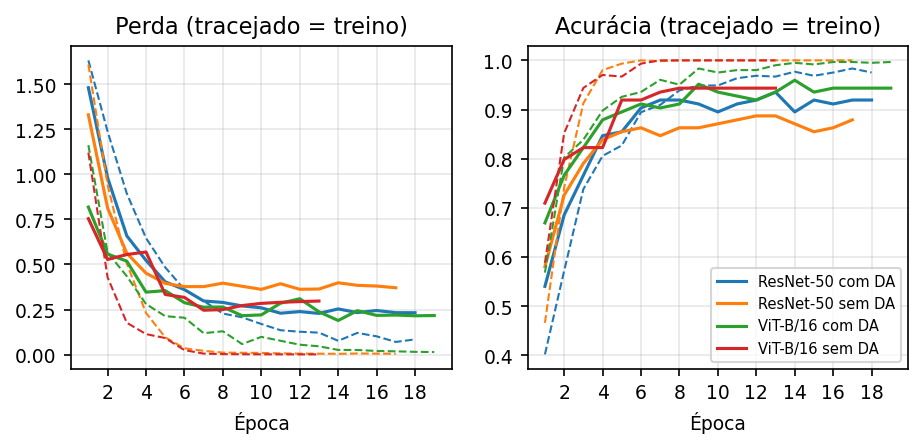
\includegraphics[width=0.85\textwidth]{figures/curves_all.png}
\caption{Perda e acurácia de treino (tracejado) e validação (contínuo) por época nos quatro experimentos.}
\label{fig:curvas}
\end{figure*}

\begin{figure*}[t]
\centering
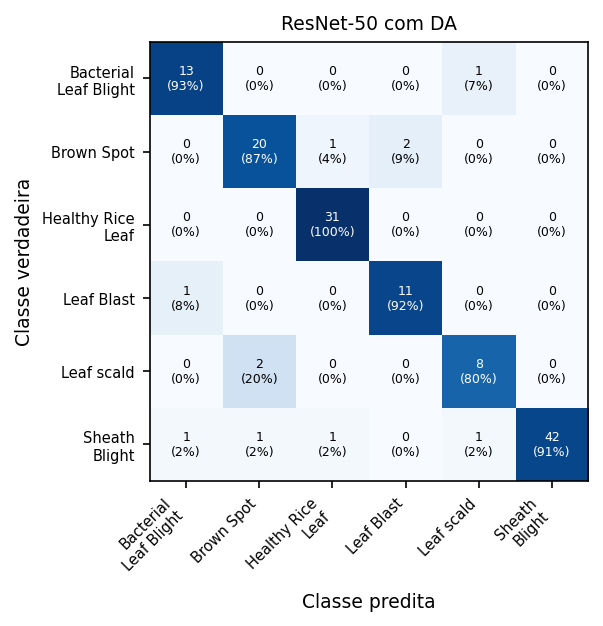
\includegraphics[width=0.40\textwidth]{figures/cm_resnet50_aug.png}\hfill
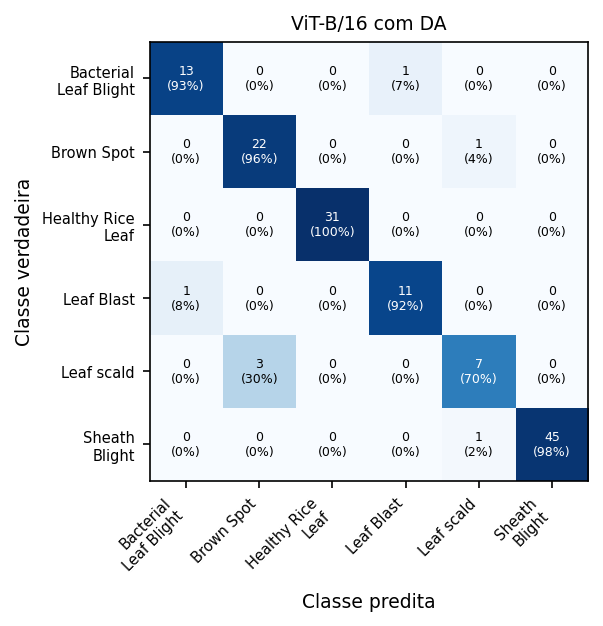
\includegraphics[width=0.40\textwidth]{figures/cm_vit_b_16_aug.png}
\caption{Matrizes de confusão no conjunto de teste para ResNet-50 (esq.) e ViT-B/16 (dir.), ambos com \textit{data augmentation}. Cada célula mostra a contagem e a porcentagem em relação à classe verdadeira.}
\label{fig:cm}
\end{figure*}

\begin{table}[t]
\centering
\caption{Métricas por classe no teste para o melhor modelo (ViT-B/16 com DA).}
\label{tab:porclasse}
\begin{tabular}{lcccc}
\toprule
Classe & Precisão & Recall & F1 & Suporte \\
\midrule
Bacterial Leaf Blight & 92.86 & 92.86 & 92.86 & 14 \\
Brown Spot & 88.00 & 95.65 & 91.67 & 23 \\
Healthy Rice Leaf & 100.00 & 100.00 & 100.00 & 31 \\
Leaf Blast & 91.67 & 91.67 & 91.67 & 12 \\
Leaf scald & 77.78 & 70.00 & 73.68 & 10 \\
Sheath Blight & 100.00 & 97.83 & 98.90 & 46 \\
\bottomrule
\end{tabular}
\end{table}


\textbf{Análise por classe e qualitativa.} As matrizes de confusão (Fig.~\ref{fig:cm}) e a Tabela~\ref{tab:porclasse} mostram que a confusão mais frequente do melhor modelo foi entre \TopConfTrue{} (classe verdadeira) e \TopConfPred{} (classe predita), com \TopConfN{} ocorrências. A \textit{Leaf Scald}, classe com menos imagens (\,76 no total e apenas 10 no teste), teve o pior F1 (73,68\%), enquanto \textit{Healthy Rice Leaf} e \textit{Sheath Blight} ficaram próximas de 100\%. As duas doenças confundidas produzem lesões amarronzadas sobre folhas amareladas, e em estágios iniciais a escaldadura pode aparecer como pequenas manchas isoladas, muito semelhantes às da mancha-parda. Além disso, \NCommonErrors{} imagens de teste foram classificadas incorretamente por ambos os modelos com \textit{data augmentation}, o que sugere que esses casos são intrinsecamente difíceis e não um defeito de uma arquitetura específica.

A Fig.~\ref{fig:qualitativa} mostra exemplos de acertos e os erros de maior confiança. Nos erros observam-se três padrões. (i)~Nas imagens de \textit{Leaf Scald} preditas como \textit{Brown Spot}, a folha exibe apenas uma ou duas manchas pequenas e arredondadas, sem o padrão de faixas na ponta da folha típico da escaldadura. (ii)~Em várias fotos a folha doente divide o quadro com muitas folhas sadias e com o solo ou a água ao fundo, de modo que a lesão ocupa poucos pixels após o redimensionamento para $224\times224$. (iii)~As confusões entre \textit{Leaf Blast} e \textit{Bacterial Leaf Blight} envolvem lesões alongadas com bordas amareladas, característica comum às duas doenças. Também não se pode descartar que algumas fotos contenham mais de uma doença ou tenham rótulo incorreto. Erros cometidos com alta confiança merecem atenção especial, pois em um sistema real não seriam sinalizados para revisão humana.

\begin{figure*}[t]
\centering
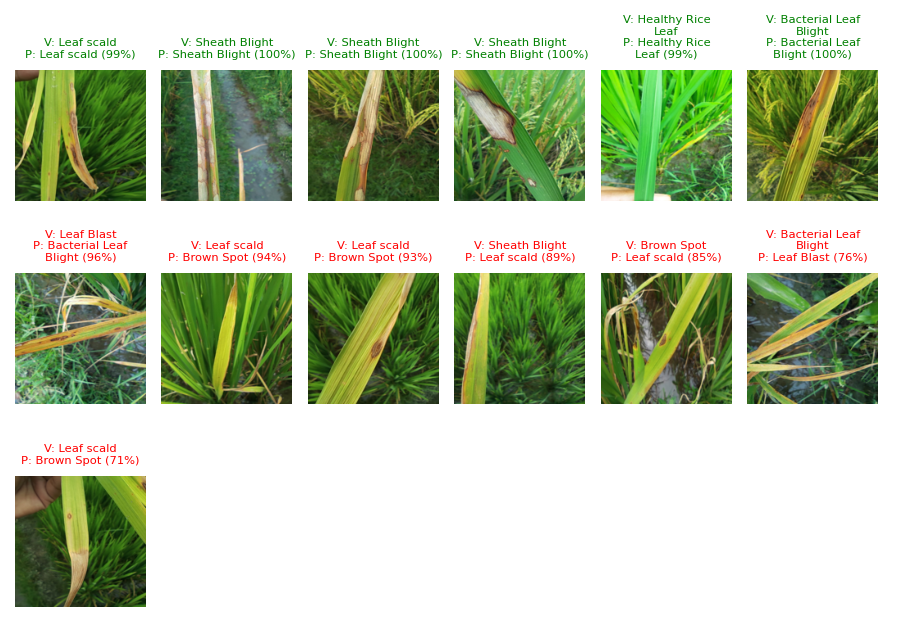
\includegraphics[width=0.85\textwidth]{figures/qualitative_best.png}
\caption{Análise qualitativa do melhor modelo (\BestLabel{}). Primeira linha: acertos (verde). Demais linhas: erros (vermelho), ordenados pela confiança. V = classe verdadeira; P = classe predita (probabilidade).}
\label{fig:qualitativa}
\end{figure*}

\textbf{Limitações.} Os resultados vêm de uma única divisão \textit{hold-out} e de uma única semente, de modo que diferenças de poucos pontos percentuais entre os modelos correspondem a poucas imagens e podem não ser estatisticamente significativas; repetir os experimentos com várias sementes ou validação cruzada daria uma estimativa mais robusta. Além disso, o agrupamento por \textit{hash} perceptual detecta cópias redimensionadas, recomprimidas, giradas em múltiplos de $90^\circ$ ou espelhadas, mas não fotos diferentes da mesma folha tiradas de ângulos distintos. Por fim, o descarte das imagens aumentadas reduziu o conjunto a \NClean{} fotos, o que limita o número de exemplos de teste por classe.

% =====================================================================
\section{Conclusão}\label{sec:conclusao}
Este trabalho comparou uma CNN (ResNet-50) e um \textit{Vision Transformer} (ViT-B/16), ambos com \textit{transfer learning} do ImageNet, na classificação de seis condições de folhas de arroz, avaliando também o efeito do \textit{data augmentation}. Com um protocolo controlado, com descarte das cópias aumentadas já presentes no conjunto, divisão estratificada por grupos de quase-duplicatas e teste usado apenas na avaliação final, o melhor modelo foi o \BestLabel{}, com F1-macro de \BestFOne\%. Quanto a Q1, o \textit{Vision Transformer} superou a CNN nas duas condições, ao custo de cerca de 3,6 vezes mais parâmetros, embora a diferença corresponda a poucas imagens de teste. Quanto a Q2, o \textit{data augmentation} melhorou as duas arquiteturas (\DeltaAugResNet{} e \DeltaAugViT{} p.p. de F1-macro) ao reduzir o sobreajuste. Destaca-se ainda que o conjunto público mistura fotos originais e cópias aumentadas, e que tratá-las é essencial para uma avaliação honesta. As confusões remanescentes concentram-se em doenças com sintomas visualmente semelhantes.

Como trabalhos futuros, sugerem-se: validação cruzada com múltiplas sementes e testes estatísticos; uso de técnicas de explicabilidade, como Grad-CAM, para verificar se os modelos se baseiam nas lesões; detecção de quase-duplicatas por \textit{hashing} perceptual; avaliação em imagens de outras fontes para medir a generalização; e investigação de modelos leves, como MobileNet e EfficientNet, voltados a dispositivos móveis.

\bibliographystyle{IEEEtran}
\bibliography{refs}

\end{document}
